\begin{description}
\item[1] \textit{ Give an upper bound on the number of different states a mazeCollect problem of size $n \times m$ with $k$ money items to collect ? Justify your answer precisely.}\\


Upper bound : $(n\times m) * 2^k$. 
\begin{proof}[$2^k$]
A money displayed can have two states. The characted already reached it or not. To represent all the possible combinations for the money on the board, we have $2^k$
\end{proof}
\begin{proof}[$n\times m$]
It represents all possible positions of the character.
\end{proof}
If we put this justifications together, we have the upper bound shown above. We must put together all the possible states for money and character position.


\item [2] \textit{Describe your best consistent heuristic for the mazeCollect problem. When using distance, precise which distance you use. Justify precisely the admissibility and the consistency of your heuristic.}\\

Our heuristic computes the sum of manhattan distance (shortest way) between all non-taken dollars (and the goal if all dollars are taken) and manhattan distance between our current position and closest dollar. 
\begin{proof}[Admissibility]
$h(n) \leq realCost(n)$ : it only uses manhattan distance between dollars, current position and goal. The cost computed is the minimal expected. The value computed is the real cost if there are no walls, it's optimistic if there are walls. \\
$h(n) > 0$ if n is not the goal : the distance between goal and current position is at least $1$ so $h(n) > 0$\\
\end{proof}
\begin{proof}[Consistency]

We have to prove that $h(n)\leq c(n,a,n') + h(n')$ . \\
Since the cost of moving from current position to closest dollar decreased from $1$ after an action $a$, the cost computed for successor is the cost of current state minus one. Actually, we have $h(n)= c(n,a,n') + h(n')$, with $ c(n,a,n')=1$ and $h(n')= h(n) - 1 $.

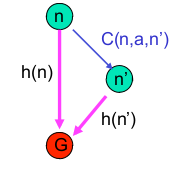
\includegraphics[scale=0.8]{consis.png}\\
\end{proof}


\item [3] \textit{Implement the first version of your solver. For this version, the moves considered in your successor function must correspond to the atomic player moves (up,right, down and left). Extend the Problem class and implement the necessary methods and other class(es) if necessary. Your program file must be named mazeCollect.py. Your program must print to the standard output a solution to the mazeCollect instance for which the path to the instance file is given in argument. This solution must satisfy the described format.} \\

\end{description}
\lstinputlisting{../mazeCollect.py} 
\begin{description}
\item [4] \textit{Experiment, compare and analyze informed (astar\_graph\_search) and uninformed (breadth\_first\_graph\_search) graph search of aima-python3 on the 10 instances of mazeCollect inside Benchs\_Small. Report in a table the time, the number of explored nodes and the number of steps to reach the solution. Be aware that the last two instances can only be solved using $A^\ast$ with a good heuristic. When no solution can be found by a strategy in a reasonable time (say 3 min), explain the reason (time-out and/or swap of the memory).} \\

\begin{tabular}{|c|c|c|c|c|c|c|} \hline  mazeCollect.py & \multicolumn{3}{c|}{BFS} & \multicolumn{3}{c|}{$A^\ast search$} \\ 
\hline Benchs\_Small & Time (s.) & Explored nodes & Steps & Time (s.) & Explored nodes & Steps \\ \hline 
mazeCollect0 & 0,74 & 27.761 & 76 & 0,63 & 10.200 & 76\\
mazeCollect1 & 0,34 & 11.917 & 70 & 0,64 & 10.636 & 70 \\  
mazeCollect2 & 6,53 & 180.602 & 84 & 3,33 & 43.979 & 84\\
mazeCollect3 & 0,93 & 35.789 & 103 & 0,83 & 14.160 & 103\\
mazeCollect4 & 5,48 & 169.287 & 99 & 6,38 & 86.559 & 99\\
mazeCollect5 & 9,68 & 283.145 & 132 & 15,37 & 188.149 & 132 \\
mazeCollect6 & 12,78 & 335.952 & 123 & 6,83 & 91.388 & 123\\
mazeCollect7 & 8,89 & 253.242 & 158 & 11,99 & 158.156 & 158\\
mazeCollect8 & 43,02 & 1.020.263 & 103 & 88,09 & 498.016 & 103\\
mazeCollect9 & 75,02 & 1.530.281 & 245 & 26.17 & 255.260 & 245\\
\hline
\end{tabular}\\

\item [5] \textit{In your experiments, is the time taken by $A^\ast$ always smaller than the one taken by breadth first search and why ?} \\

No, it depends on the cases. Because of errors from heuristic (too optimistic), $A^\ast$ can try to search in a way it will be stucked by walls. The time used to compute manhattan distance between all the elements explained earlier can take several time. This time is lost if the subtree chosen by the heuristic seems finally not being an optimal one. BFS make a way less computations even if it goes through many more nodes.

\item [6] In your experiments, is the number of nodes explored by $A^\ast$ always smaller than the number of nodes explored by breadth first search and why ? \\
Yes, it is very logical. BFS try to search in all nodes, even the ones describing a very bad move. During this time, $A^\ast$ chooses only nodes which seems to do good moves. 



\end{description}